\sectionquestion{MDPs and Value/Policy Iteration}

\begin{parts}

\newcommand{\mya}{ \text{\color{blue}$\blacksquare$} }
\newcommand{\myb}{ \text{\color{red}$\blacktriangle$} }

\part[2] \textbf{True or False:} For a given Markov decision process (MDP), is the optimal policy unique? \textbf{Briefly justify your answer.}
    \begin{checkboxes}
     \choice Yes 
     \choice No
    \end{checkboxes}
    \fillwithlines{8em}
    \begin{soln}
    No, there may be multiple actions at a given state that have the same optimal value and therefore we can have multiple optimal policies for a given MDP.
    \end{soln}
    \begin{qauthor}    Matt    \end{qauthor}
    
\part[1] \textbf{Fill in the blanks:} Value iteration can be viewed as an application of the \underline{\qquad} algorithm to the \underline{\qquad}.
    \begin{checkboxes}
     \choice block coordinate descent; Bellman equations for the model policy
     \choice block coordinate descent; optimal value function equations
     \choice fixed point iteration; Bellman equations for the model policy
     \choice fixed point iteration; optimal value function equations
    \end{checkboxes}
    \begin{soln}
    fixed point iteration; optimal value function
    \end{soln}
    \begin{qauthor}    Matt    \end{qauthor}

\part Below we define a Markov decision process (MDP) as a finite state machine. 
\begin{center}
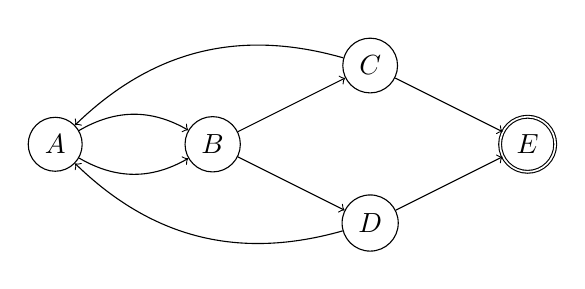
\begin{tikzpicture}
  % Nodes
  \node[circle, draw] (A) at (0,0) {$A$};
  \node[circle, draw] (B) at (2,0) {$B$};
  \node[circle, draw] (C) at (4,1) {$C$};
  \node[circle, draw] (D) at (4,-1) {$D$};
  \node[circle, draw, double] (E) at (6,0) {$E$};
  % Edges
  \draw[->, bend left] (A) to node[] {\mya} (B);
  \draw[->, bend right] (A) to node[] {\myb} (B);
  \draw[->] (B) to node[] {\mya} (C);
  \draw[->] (B) to node[] {\myb} (D);
  \draw[->] (C) to node[] {\mya} (E);
  \draw[->, bend right] (C) to node[] {\myb} (A);
  \draw[->, bend left] (D) to node[] {\mya} (A);
  \draw[->] (D) to node[] {\myb} (E);
\end{tikzpicture}
\end{center}
Each state in the state space $\Sc = \{A, B, C, D, E\}$ is represented by a node. The action space $\Ac = \{\mya, \myb\}$ contains two actions. 
%
We assume deterministic transitions. The transition function $s' = \delta(s, a)$ is represented by the outgoing edges from each node; e.g., from state $B$ taking action $\mya$ will transition to $C$, and taking action $\myb$ will transition to $D$. 
%\tikz{ \draw[->] (0,0) to node[] {\mya}  (1,0); } 
%
The reward function is:
\begin{align*}
    R(s, a) = \begin{cases}
    16 & \text{if } s = C \text{ and } a = \mya \\
    8 & \text{if } s = D \text{ and } a = \myb \\
    -2 & \text{otherwise}
    \end{cases}
\end{align*}
%
Assume a discount factor of $0.5$. 
%
The state $E$ is terminal.

\clearpage

\begin{subparts}

\subpart[2] \textbf{Numerical answer:} After the \textbf{first} iteration of synchronous value iteration, what are the following $V$ table values? Assume the $V$ table is initialized to all zeros.

    $V(A) = $
    \begin{tcolorbox}[fit,height=1cm, width=2cm, blank, borderline={1pt}{-2pt}, nobeforeafter]
    %solution
    \end{tcolorbox}
    \hspace{1em}
    $V(B) = $
    \begin{tcolorbox}[fit,height=1cm, width=2cm, blank, borderline={1pt}{-2pt}, nobeforeafter]
    %solution
    \end{tcolorbox}
    \hspace{1em}
    $V(C) = $
    \begin{tcolorbox}[fit,height=1cm, width=2cm, blank, borderline={1pt}{-2pt}, nobeforeafter]
    %solution
    \end{tcolorbox}
    
    \begin{soln}
    $V(A) = R(A, \mya) + 0.5 * V(B) = -2$ \\
    $V(B) = R(B, \mya) + 0.5 * V(C) = -2$ \\
    $V(C) = R(C, \mya) + 0.5 * V(E) = 16$ \\
    \end{soln}
    \begin{qauthor}    Matt    \end{qauthor}
    
\subpart[2] \textbf{Numerical answer:} After the \textbf{second} iteration of synchronous value iteration, what are the following $V$ table values? Assume the $V$ table is initialized to all zeros.

    $V(A) = $
    \begin{tcolorbox}[fit,height=1cm, width=2cm, blank, borderline={1pt}{-2pt}, nobeforeafter]
    %solution
    \end{tcolorbox}
    \hspace{1em}
    $V(B) = $
    \begin{tcolorbox}[fit,height=1cm, width=2cm, blank, borderline={1pt}{-2pt}, nobeforeafter]
    %solution
    \end{tcolorbox}
    \hspace{1em}
    $V(C) = $
    \begin{tcolorbox}[fit,height=1cm, width=2cm, blank, borderline={1pt}{-2pt}, nobeforeafter]
    %solution
    \end{tcolorbox}
    
    \begin{soln}
    $V(A) = R(A, \mya) + 0.5 * V(B) = -2 + -1 = -3$ \\
    $V(B) = R(B, \mya) + 0.5 * V(C) = -2 + 8 = 6$ \\
    $V(C) = R(C, \mya) + 0.5 * V(E) = 16$ \\
    \end{soln}
    \begin{qauthor}    Matt    \end{qauthor}

\uplevel{Now consider a modified version of this MDP where each transition is stochastic. With probability $0.75$ we transition to the node at the end of the outgoing edge marked with the action taken, and with probability $0.25$ we transition to the node along the other outgoing arrow, e.g. $p(C \mid B, \mya) = 0.75$ and $p(D \mid B, \mya) = 0.25$ }


\subpart[2] \textbf{Short answer:} In this nondeterministic setting, how does synchronous value iteration recompute the value of $V^{(t+1)}(C)$? Write your answer \textbf{only} in terms of $R(A, \mya), R(A, \myb), \ldots, R(E, \mya), R(E, \myb)$ and $V^{(t)}(A), V^{(t)}(B), \ldots, V^{(t)}(E)$ and the function $\max(\ldots)$ and any numerical constants you may need. 
    \begin{tcolorbox}[fit,height=2cm, width=15cm, blank, borderline={1pt}{-2pt}]
    %solution
    \end{tcolorbox}
    \begin{soln}
    \begin{align*}
    V(C) = \max(  
    & R(C, \mya) + 0.5 * (0.75 * V(E) + 0.25 * V(A)), \\
    & R(C, \myb) + 0.5 * (0.25 * V(E) + 0.75 * V(A)) )
    \end{align*}
    \end{soln}
    \begin{qauthor}    Matt    \end{qauthor}

\subpart[2] \textbf{Numerical answer:} In this nondeterministic setting, after the \textbf{second} iteration of synchronous value iteration, what are the following $V$ table values? Assume the $V$ table is initialized to all zeros.

    $V(A) = $
    \begin{tcolorbox}[fit,height=1cm, width=2cm, blank, borderline={1pt}{-2pt}, nobeforeafter]
    %solution
    \end{tcolorbox}
    \hspace{2em}
    $V(C) = $
    \begin{tcolorbox}[fit,height=1cm, width=2cm, blank, borderline={1pt}{-2pt}, nobeforeafter]
    %solution
    \end{tcolorbox}

    \textit{(You may show your work in the box below. We will only inspect this box if you do {not} get the numerical answers above correct.)}
    \begin{tcolorbox}[fit,height=5cm, width=15cm, blank, borderline={1pt}{-2pt}]
    %solution
    \end{tcolorbox}
    
    \begin{soln}
    $V(A) = -3; V(C) = 15.75$ (or $V(C) = 14.25$ if assuming E has a single "stay put" action) \\
    First iteration: \\
    $V(A) = R(A, \mya) + 0.5 * V(B) = -2 $ \\
    $V(B) = R(B, \mya) + 0.5 * (0.75 * V(C) + 0.25 * V(D)) = -2$ \\
    $V(C) = R(C, \mya) + 0.5 * (0.75 * V(E) + 0.25 * V(A)) = 16$ \\
    $V(D) = R(B, \mya) + 0.5 * (0.75 * V(E) + 0.25 * V(A)) = 8$ \\
    $V(E) = 0$ b/c terminal (or $V(E) = -2$ b/c stay put action.)
    Second iteration: \\
    $V(A) = R(A, \mya) + 0.5 * V(B) = -2 + 0.5 * -2 $ \\
    $V(B) = R(B, \mya) + 0.5 * (0.75 * V(C) + 0.25 * V(D)) = -2 + 0.5 * (0.75*16 + 0.25*8)$ \\
    $V(C) = R(C, \mya) + 0.5 * (0.75 * V(E) + 0.25 * V(A)) = 16 + 0.5*(0 + 0.25*-2)$ \\
    $V(D) = R(B, \mya) + 0.5 * (0.75 * V(E) + 0.25 * V(A)) = 16 + 0.5*(0 + 0.25*-2)$ \\
    \end{soln}
    \begin{qauthor}    Matt    \end{qauthor}
    
\end{subparts}

\end{parts}